

\section{Additional Analysis of Negative-Advantage Veto and Relaxed Clipping}
\label{app:nav_relaxed_clipping}

This section provides additional analyses and ablations for the two stabilization
components of \ourmethod{}: negative-advantage veto (NAV) and relaxed clipping.
We first analyze how often NAV vetoes token-level updates during training, then
compare different NAV masking scopes, study the sensitivity to the NAV threshold
and clipping upper bound, and finally test whether the \ourmethod{} update rule
remains compatible with the standard low-staleness regime.

\subsection{Fraction of Tokens Vetoed by NAV}
\label{app:veto_fraction}

To better understand how much training signal is filtered by NAV, we report the fraction of tokens vetoed during \ourmethod{} training. Recall that under the sequence-level NAV rule, for a negative-advantage response, once a token's importance ratio falls below the threshold $\tau_c$, NAV masks all remaining tokens in the response after the trigger. We define the NAV-vetoed token fraction as the number of tokens masked by NAV divided by the total number of tokens in the optimization batch. Since NAV masks are recomputed online during optimization, this fraction can vary across updates within a stage. These statistics correspond to the main \ourmethod{} runs reported in Table~\ref{tab:performance_comparison}.

\begin{table}[!h]
\vspace{-8pt}
\centering
\caption{Mean NAV-vetoed token fraction in each stage, computed as vetoed tokens
divided by all tokens in the optimization batch. Avg. is the unweighted average
across stages.}
\label{tab:veto_fraction}
\begin{tabular}{lccccc}
\toprule
Model & Stage 0 & Stage 1 & Stage 2 & Stage 3 & Veto Avg. \\
\midrule
Llama-3.2-3B-Instruct & 6.08\% & 3.28\% & 0.78\% & 2.42\% & 3.14\% \\
Qwen2.5-Math-7B & 15.24\% & 0.27\% & 0.27\% & 0.32\% & 4.03\% \\
Qwen3-Base-1.7B & 7.07\% & 0.22\% & 0.23\% & 0.42\% & 1.99\% \\
Qwen3-Base-8B & 3.78\% & 0.81\% & 2.83\% & 4.72\% & 3.04\% \\
DeepSeek-7B & 0.61\% & 0.01\% & 0.01\% & 0.05\% & 0.17\% \\
\bottomrule
\end{tabular}
\vspace{-1pt}
\end{table}

Table~\ref{tab:veto_fraction} reports the mean NAV-vetoed token fraction in each stage for all five models, along with the unweighted average across stages. Overall, the average vetoed fraction remains small, ranging from 0.17\% on DeepSeek-7B to 4.03\% on Qwen2.5-Math-7B. This shows that NAV removes only a limited subset of token-level updates rather than discarding a large portion of the rollout data. The result supports the view that NAV primarily suppresses harmful off-support negative-advantage updates while preserving most of the training signal.  

The vetoed fraction is especially small in later stages. For Qwen2.5-Math-7B, the mean vetoed token fraction is 15.24\% in Stage 0 but drops to below 0.4\% in all subsequent stages. Similarly, Qwen3-Base-1.7B decreases from 7.07\% in Stage 0 to below 0.5\% afterward, while DeepSeek-7B remains below 0.7\% across all stages. These trends suggest that NAV is most active when the model is early in training or when the rollout distribution is more prone to off-support negative-advantage updates, and becomes increasingly sparse once the staged training process stabilizes.

\begin{figure*}[!h]
\vspace{-5pt}
\centering
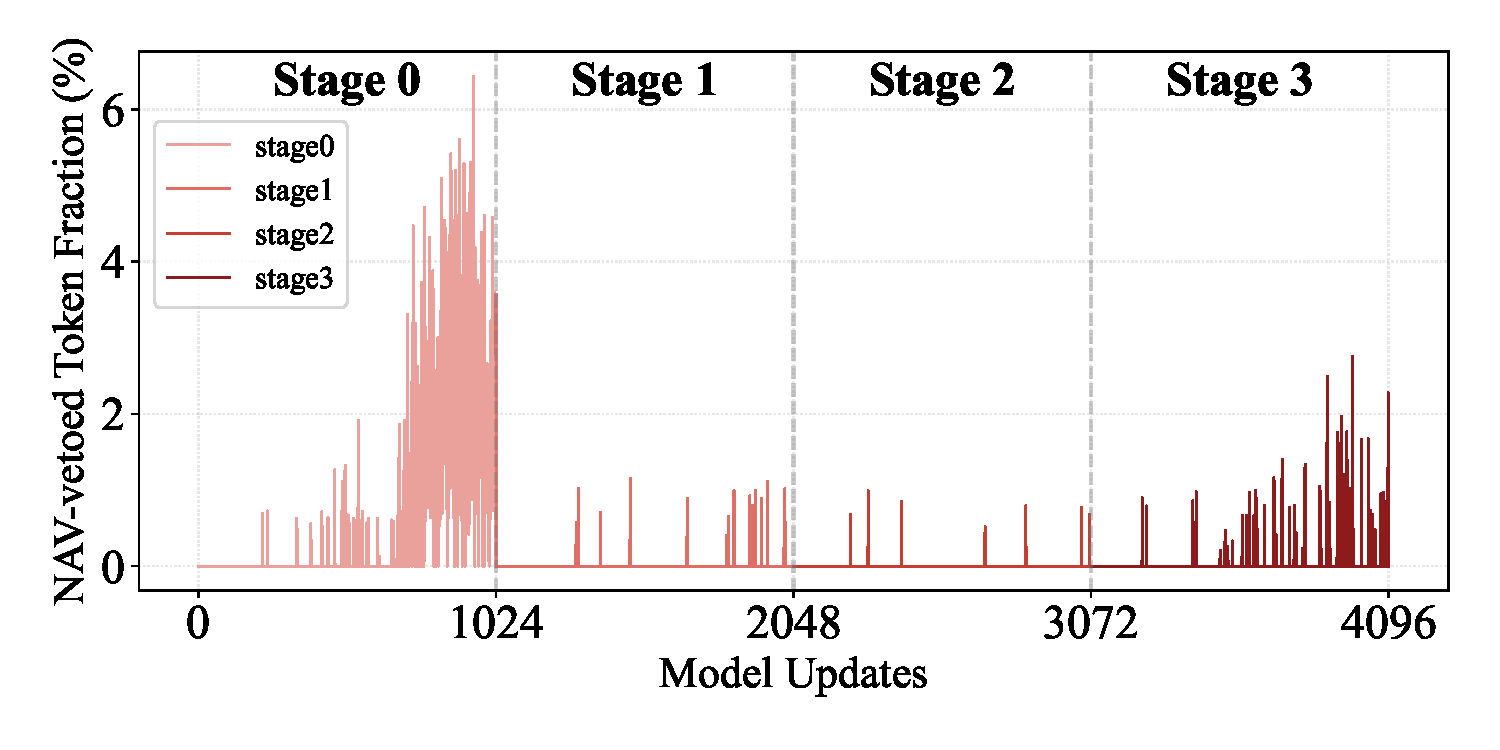
\includegraphics[width=0.6\textwidth]{figures/veto_frac.pdf}
\vspace{-12pt}
\caption{NAV-vetoed token fraction during $\mu$-GRPO training on DeepSeek-7B.}
\label{fig:veto_frac}
\vspace{-16pt}
\end{figure*}

To complement the averages in Table~\ref{tab:veto_fraction},
Figure~\ref{fig:veto_frac} visualizes the NAV-vetoed token fraction throughout
training for DeepSeek-7B across the four stages. The curve shows that the vetoed
token fraction remains close to zero for most updates, with only occasional peaks
within individual stages. Overall, these results show that NAV stabilizes high-staleness training through sparse token-level intervention.

\subsection{NAV Scope Ablation}
\label{app:nav_scope_ablation}

In the main experiments, we use the sequence-level NAV scope $\mathcal S_{\mathrm{seq}}$ as the default choice. For a negative-advantage response, once a token with importance ratio below $\tau_c$ is detected, it vetoes all tokens in that response. The diagnostic experiments in Section~\ref{sec:diagnosis} identify the post-boundary harmful suffix $\mathcal H_\kappa$ as the critical subset that must be removed to prevent collapse. This suggests that masking scopes that include $\mathcal H_\kappa$, such as $\mathcal S_{\kappa}$ and $\mathcal S_{\mathrm{seq}}$, should also stabilize high-staleness optimization.

To examine the effect of the veto scope, we compare three NAV scopes under the main experimental setting: 4096 model updates with four rollout stages, corresponding to $\mu=1024$ updates per stage. The scopes are the minimal harmful suffix $\mathcal H_\kappa$, the full post-boundary
suffix $\mathcal S_{\kappa}$, and the sequence-level scope
$\mathcal S_{\mathrm{seq}}$. We report
the fraction of vetoed tokens in each stage, computed as the number of vetoed
tokens divided by the total number of tokens in the optimization batch. We also
report the average veto rate across stages and the average accuracy across the five math benchmarks.

\begin{table}[!h]
\vspace{-8pt}
\centering
\caption{NAV scope ablation on Qwen2.5-Math-7B. Veto rates are reported per stage.}
\label{tab:nav_scope_ablation}
\begin{tabular}{ccccccc}
\toprule
NAV Scope & Stage 0 & Stage 1 & Stage 2 & Stage 3 & Veto Avg. & Avg. Acc. \\
\midrule
$\mathcal H_\kappa$
& 11.70\% & 0.18\% & 0.21\% & 0.17\% & 3.07\% & 47.9 \\
$\mathcal S_{\kappa}$
& 13.40\% & 0.22\% & 0.23\% & 0.22\% & 3.52\% & {47.6} \\
\rowcolor{gray!20}
$\mathcal S_{\mathrm{seq}}$ 
& 15.24\% & 0.27\% & 0.27\% & 0.32\% & 4.03\% & \textbf{48.0} \\
\bottomrule
\end{tabular}
\vspace{-2pt}
\end{table}

All three scopes remain stable and achieve similar average accuracy. The minimal scope $\mathcal H_\kappa$ vetoes the fewest tokens, whereas $\mathcal S_{\mathrm{seq}}$ vetoes the most because it removes the entire negative-advantage response once a trigger is detected. The comparison suggests that the additional prefix tokens retained by $\mathcal H_\kappa$ and $\mathcal S_{\kappa}$ provide limited benefit once a trigger has appeared. Since the response has negative advantage and has already crossed an off-support boundary under the current policy, the remaining useful contribution from the pre-trigger prefix is small compared with the risk of continuing to update on the same trajectory. Consistent with this view, the more conservative sequence-level scope achieves the best average accuracy despite vetoing more tokens. We therefore use $\mathcal S_{\mathrm{seq}}$ in the main experiments because it is simple, robust, and slightly outperforms the other scopes in this ablation.

\subsection{Stabilization Hyperparameter Sensitivity}
\label{app:stabilization_hyperparams}

We study the sensitivity of \ourmethod{} to two stabilization-related hyperparameters: the NAV threshold $\tau_c$ and the relaxed clipping upper bound. All experiments follow the main experimental setting: Qwen2.5-Math-7B is trained for 4096 model updates with four rollout stages, corresponding to $\mu=1024$ updates per stage. We report the average accuracy across the five math benchmarks.

\paragraph{NAV Threshold Sensitivity.}
The NAV threshold $\tau_c$ determines when a negative-advantage response is treated as crossing the off-support boundary and triggers sequence-level vetoing. Since this threshold is intended to detect extreme low-ratio events, it should be sufficiently small; an overly large threshold may trigger NAV prematurely and remove useful updates.

\begin{table}[!h]
\vspace{-10pt}
\centering
\small
\caption{NAV threshold sensitivity.}
\label{tab:nav_threshold_ablation}
\begin{tabular}{cc}
\toprule
NAV threshold $\tau_c$ & Avg. Acc. \\
\midrule
$10^{-1}$ & 45.2 \\
$10^{-2}$ & 46.4 \\
\rowcolor{gray!20}
$10^{-4}$ & \textbf{48.0} \\
$10^{-6}$ & 47.6 \\
\bottomrule
\end{tabular}
\vspace{-11pt}
\end{table}

We sweep $\tau_c$ over $\{10^{-1}, 10^{-2}, 10^{-4}, 10^{-6}\}$. As shown in Table~\ref{tab:nav_threshold_ablation}, $\tau_c=10^{-4}$ achieves the best average accuracy of 48.0\%, while $10^{-6}$ remains close at 47.6\%. In contrast, larger thresholds degrade performance, with $10^{-1}$ dropping to 45.2\%. These results suggest that NAV is robust once the threshold is small enough, but setting it too large can over-veto negative-advantage responses before they truly indicate an off-support boundary.

\paragraph{Clipping Upper Bound Sensitivity.}
We also ablate the upper bound of the relaxed clipping interval. In
high-staleness training, the standard GRPO clipping range can overly suppress useful gradients from stale but still informative rollouts.
\ourmethod{} therefore uses a relaxed clipping range, while relying on NAV to remove destabilizing negative-advantage suffix updates.
\begin{table}[!h]
\vspace{-11pt}
\centering
\small
\caption{Clipping upper bound sensitivity.}
\label{tab:clip_upper_ablation}
\begin{tabular}{cc}
\toprule
Clipping upper bound & Avg. Acc. \\
\midrule
3 & 47.3 \\
\rowcolor{gray!20}
5 & 48.0 \\
10 & 47.8 \\
$+\infty$ & 43.6 \\
\bottomrule
\end{tabular}
\vspace{-3pt}
\end{table}
With the staged pipeline fixed, we vary the clipping upper bound over
$\{3, 5, 10, +\infty\}$, where $+\infty$ denotes no upper clipping. Table~\ref{tab:clip_upper_ablation} shows that an upper bound of 5 achieves the best average accuracy, reaching 48.0\%. A tighter bound of 3 slightly underperforms at 47.3\%, suggesting that it still restricts some useful stale-rollout gradients. Increasing the bound to 10 gives comparable  performance at 47.8\%. Removing the upper bound entirely leads to a clear drop to 43.6\%, showing that although relaxed clipping is beneficial, some upper bound control remains necessary for stable optimization. Thus, a moderately relaxed upper bound best balances useful stale-rollout gradients and stability.

\subsection{Low-Staleness \boldmath{\ourmethod}}
\label{app:onpolicy_relaxed_nav}

We further test whether the \ourmethod{} update rule is compatible with the standard low-staleness regime. Specifically, we run \ourmethod{} with $\mu=4$, matching the rollout refresh frequency of standard GRPO while enabling the relaxed clipping range $[0,5]$ and NAV. This isolates the effect of the update rule from large-staleness rollout reuse. We report the average accuracy across the five math benchmarks and the average token clipping fraction during training.

\begin{table}[tbh]
% \tabcolsep 4.5pt
\vspace{-10pt}
\caption{Low-staleness $\mu$-GRPO on Qwen2.5-Math-7B.}
  \label{tab:onpolicy_relaxed_nav}
  \centering
  \small
\begin{sc}
  \begin{tabular}{c|c|ccccc|cc}
    \toprule
    Methods & $\mu$
    & AMC23 & AMC24
    & AIME24 & AIME25
    & Math500
    & Avg.
    & Clip Frac \\
    \midrule\midrule
    GRPO & 4
      & 68.1 & 42.8 & 29.0 & 15.8 & 81.0 & 47.3 & $4{\times}10^{-4}$ \\
    \ourmethod & 4
      & 69.2 & 42.1 & 30.1 & 14.9 & 82.3 & \textbf{47.7} & $8{\times}10^{-7}$ \\
    \bottomrule
  \end{tabular}
\end{sc}
\end{table}

As shown in Table~\ref{tab:onpolicy_relaxed_nav}, low-staleness \ourmethod{} slightly improves average accuracy over standard GRPO, from 47.3\% to 47.7\%. It also reduces the average clipping fraction from $4\times10^{-4}$ to $8\times10^{-7}$, indicating that the relaxed clipping rule avoids unnecessary clipping when rollout staleness is small. In this low-staleness setting, the NAV veto fraction remains zero throughout training, so the mild gain is primarily attributable to relaxed clipping rather than NAV intervention. These results show that the \ourmethod{} update is compatible with fresh-data learning, and suggest that the standard GRPO clipping range can be overly conservative even when rollouts are relatively fresh.

This result should not be interpreted as a comparison between on-policy and off-policy training. Rather, it shows that the optimization rule itself matters: standard low-staleness GRPO is not necessarily the strongest GRPO-style update. In the main high-staleness setting, \ourmethod{} combines this more permissive update rule with large-stage rollout reuse and NAV-based stabilization, enabling stable and efficient learning under much larger policy drift.

